% Screen driver for Richard Zach's Sets, Logic, Computation, Bengali (India).
\documentclass[screen]{../../../../sty/open-logic-book}
\usepackage[all]{nowidow}
\usepackage{fontspec}
\setmainfont{Latin Modern Roman}
\setsansfont{Latin Modern Sans}
\setmonofont{Latin Modern Mono}
\newfontfamily\latinfont{Latin Modern Roman}
% Character classes follow the accepted Bengali OpenLogic edition.
\newfontfamily\bengalifont{NotoSerifBengali-Regular.ttf}[
  Path=../../../../fonts/,Script=Bengali,Language=Bengali,
  BoldFont=NotoSerifBengali-Bold.ttf,
  ItalicFont=NotoSerifBengali-Regular.ttf,BoldItalicFont=NotoSerifBengali-Bold.ttf,
  ItalicFeatures={FakeSlant=0.15},BoldItalicFeatures={FakeSlant=0.15},
  SmallCapsFont=NotoSerifBengali-Regular.ttf]
\usepackage[Bengali,DevanagariDanDa,BasicLatin,GeneralPunctuation]{ucharclasses}
\XeTeXcharclass"200C=\BengaliClass
\XeTeXcharclass"200D=\BengaliClass
\XeTeXgenerateactualtext=1
% A character run can end outside a TeX group; do not open groups in hooks.
\setTransitionsFor{Bengali}{\bengalifont}{\latinfont}
\setTransitionsFor{DevanagariDanDa}{\bengalifont}{\latinfont}
\errorcontextlines=40
\definecolor{OLPcolor}{RGB}{151,86,7}
\definecolor{OLPdkcolor}{RGB}{104,65,6}
\definecolor{OLPltcolor}{RGB}{248,203,137}
\usepackage[nonumberlist,toc,style=index]{glossaries}
\makeglossaries
\def\oljobname{slc}
\newcommand*{\olpath}{../../../..}
\newcommand*{\ollangid}{bn}
\newcommand*{\ollanguage}{bengali}
\input{\olpath/sty/open-logic.sty}
\setOLPbooktitle[সেট, যুক্তি,\\ গণনা]{সেট, যুক্তি, গণনা}
\setOLPbooksubtitle{অধিযুক্তিবিদ্যার একটি উন্মুক্ত ভূমিকা}
\setOLPauthor{Richard Zach}
\setOLPbookversion{ভারতীয় বাংলা সংস্করণ}{বাংলা (ভারত)}
\setOLPsourcelink{https://slc.openlogicproject.org/}
\setOLPauthorlink{https://richardzach.org/}
\AtBeginDocument{%
  \renewcommand*{\olremixedby}{%
    মূল পাঠের রচয়িতা ও সংকলক: \href{\OLPauthorlink}{\OLPauthor}\par
    ওপেন লজিক প্রকল্পের পাঠের উপর ভিত্তি করে।\par\medskip
    ভারতীয় বাংলা পাঠ: OpenAI Codex-এর এআই অনুবাদ।\par
    এই পাঠ্যবইয়ের অনুবাদ, সম্পাদনা ও অক্ষরবিন্যাস:
    GPT-6.1 Sol (Ultra)।\par
    পুনর্ব্যবহৃত বাংলা ওপেন লজিক পাঠে GPT-5.6 Sol ও GPT-6 Sol-এর
    অনুবাদ এবং GPT-6.1 Sol-এর সম্পাদনা রয়েছে (Ultra)।}%
  \renewcommand*{\olcolophon}{বাংলা অক্ষর Noto Serif Bengali-তে এবং
    লাতিন অক্ষর Latin Modern-এ; গাণিতিক অক্ষর মূল বইয়ের রীতি অনুসারে।
    মুদ্রাক্ষরবিন্যাস XeLaTeX-এ।}%
  \renewcommand*{\olbookrevision}{মূল পাঠ: \href{https://github.com/rzach/sets-logic-computation/tree/6178f32f61645f3b62ef621b4c5a88f8e67778ad}{Richard Zach, \emph{Sets, Logic, Computation}}।
    ভিত্তি: \href{https://github.com/OpenLogicProject/OpenLogic/tree/9620cc73f9c8e0ad003c514a5d3748f29611c4c0}{\emph{Open Logic Text}}।
    পাঠের লাইসেন্স CC BY 4.0; প্রচ্ছদের প্রতিকৃতি ও জীবনীতে ব্যবহৃত
    আলোকচিত্রের স্বত্ব ও ব্যবহারের শর্ত পৃথক। আলোকচিত্রের স্বীকৃতি
    বইয়ের শেষে।}%
  \renewcommand*{\oluselicense}[2]{%
    \parbox[b]{.67\linewidth}{\footnotesize
      এই বইয়ের পাঠ \href{https://creativecommons.org/licenses/by/4.0/}{CC BY 4.0}
      লাইসেন্সে প্রকাশিত। এটি Richard Zach-এর \emph{Sets, Logic, Computation}
      ও ওপেন লজিক প্রকল্পের পাঠের উপর ভিত্তি করে।}\hfill
    \href{https://openlogicproject.org/}{%
      \includegraphics[width=.28\linewidth]{\olpath/assets/logos/openlogic-logo-bw}}}%
}

\input{\olpath/sty/open-logic-defer.sty}
\newcommand*{\slcbiband}{ও}
\newcommand*{\slcbibetal}{প্রমুখ}
\renewcommand*{\OLUnLocalizedHook}[1]{%
  \PackageError{slc-bn}{A native module is missing its Bengali locale identifier}{}}
% The source carries stable alphabetical sort keys independent of makeindex's locale.
\newcommand{\slcterm}[5][]{%
  \newglossaryentry{#2}{sort={#3},name={#4},description={#5},symbol={#1}}%
}

\loadglsentries{include/glossary}
\setlength{\emergencystretch}{3em}
\setlength{\headheight}{19pt}
\linespread{1.12}
\hypersetup{pdflang={bn-IN},pdfsubject={অধিযুক্তিবিদ্যার একটি উন্মুক্ত ভূমিকা},
  pdfkeywords={সেটতত্ত্ব, যুক্তিবিদ্যা, গণনসাধ্যতা, টুরিং যন্ত্র}}
\AtBeginDocument{%
  \makeoddhead{OLPpage}{\footnotesize\sffamily\color{OLPdkcolor}%
    \parbox[b]{.82\textwidth}{\raggedright\leftmark}}{}{\sffamily\bfseries\thepage}%
  \makeevenhead{OLPpage}{\footnotesize\sffamily\color{OLPdkcolor}%
    \parbox[b]{.82\textwidth}{\raggedright\leftmark}}{}{\sffamily\bfseries\thepage}%
}
\begin{document}
\raggedbottom
\OLPscreencover{%
  \centering
  \includegraphics[width=.23\textwidth]{\olpath/assets/portraits/cantor-circle.pdf}\quad
  \includegraphics[width=.23\textwidth]{\olpath/assets/portraits/goedel-circle.pdf}\quad
  \includegraphics[width=.23\textwidth]{\olpath/assets/portraits/turing-circle.pdf}\par\medskip
  \includegraphics[width=.23\textwidth]{\olpath/assets/portraits/skolem-circle.pdf}\quad
  \includegraphics[width=.23\textwidth]{\olpath/assets/portraits/noether-circle.pdf}\par
}
% Sets, Logic, Computation — chapter and appendix assembly.
\preto\OLEndChapterHook{%
  \IfFileExists{include/summary-\thechapter.tex}{%
    \section*{সারাংশ}\addcontentsline{toc}{section}{সারাংশ}%
    \let\emph\textbf\input{include/summary-\thechapter}\let\emph\textit}{}}
\problemsperchapter
\frontmatter
\OLPfrontmatter
\cleartoverso
\thispagestyle{empty}
\ \vfill
\noindent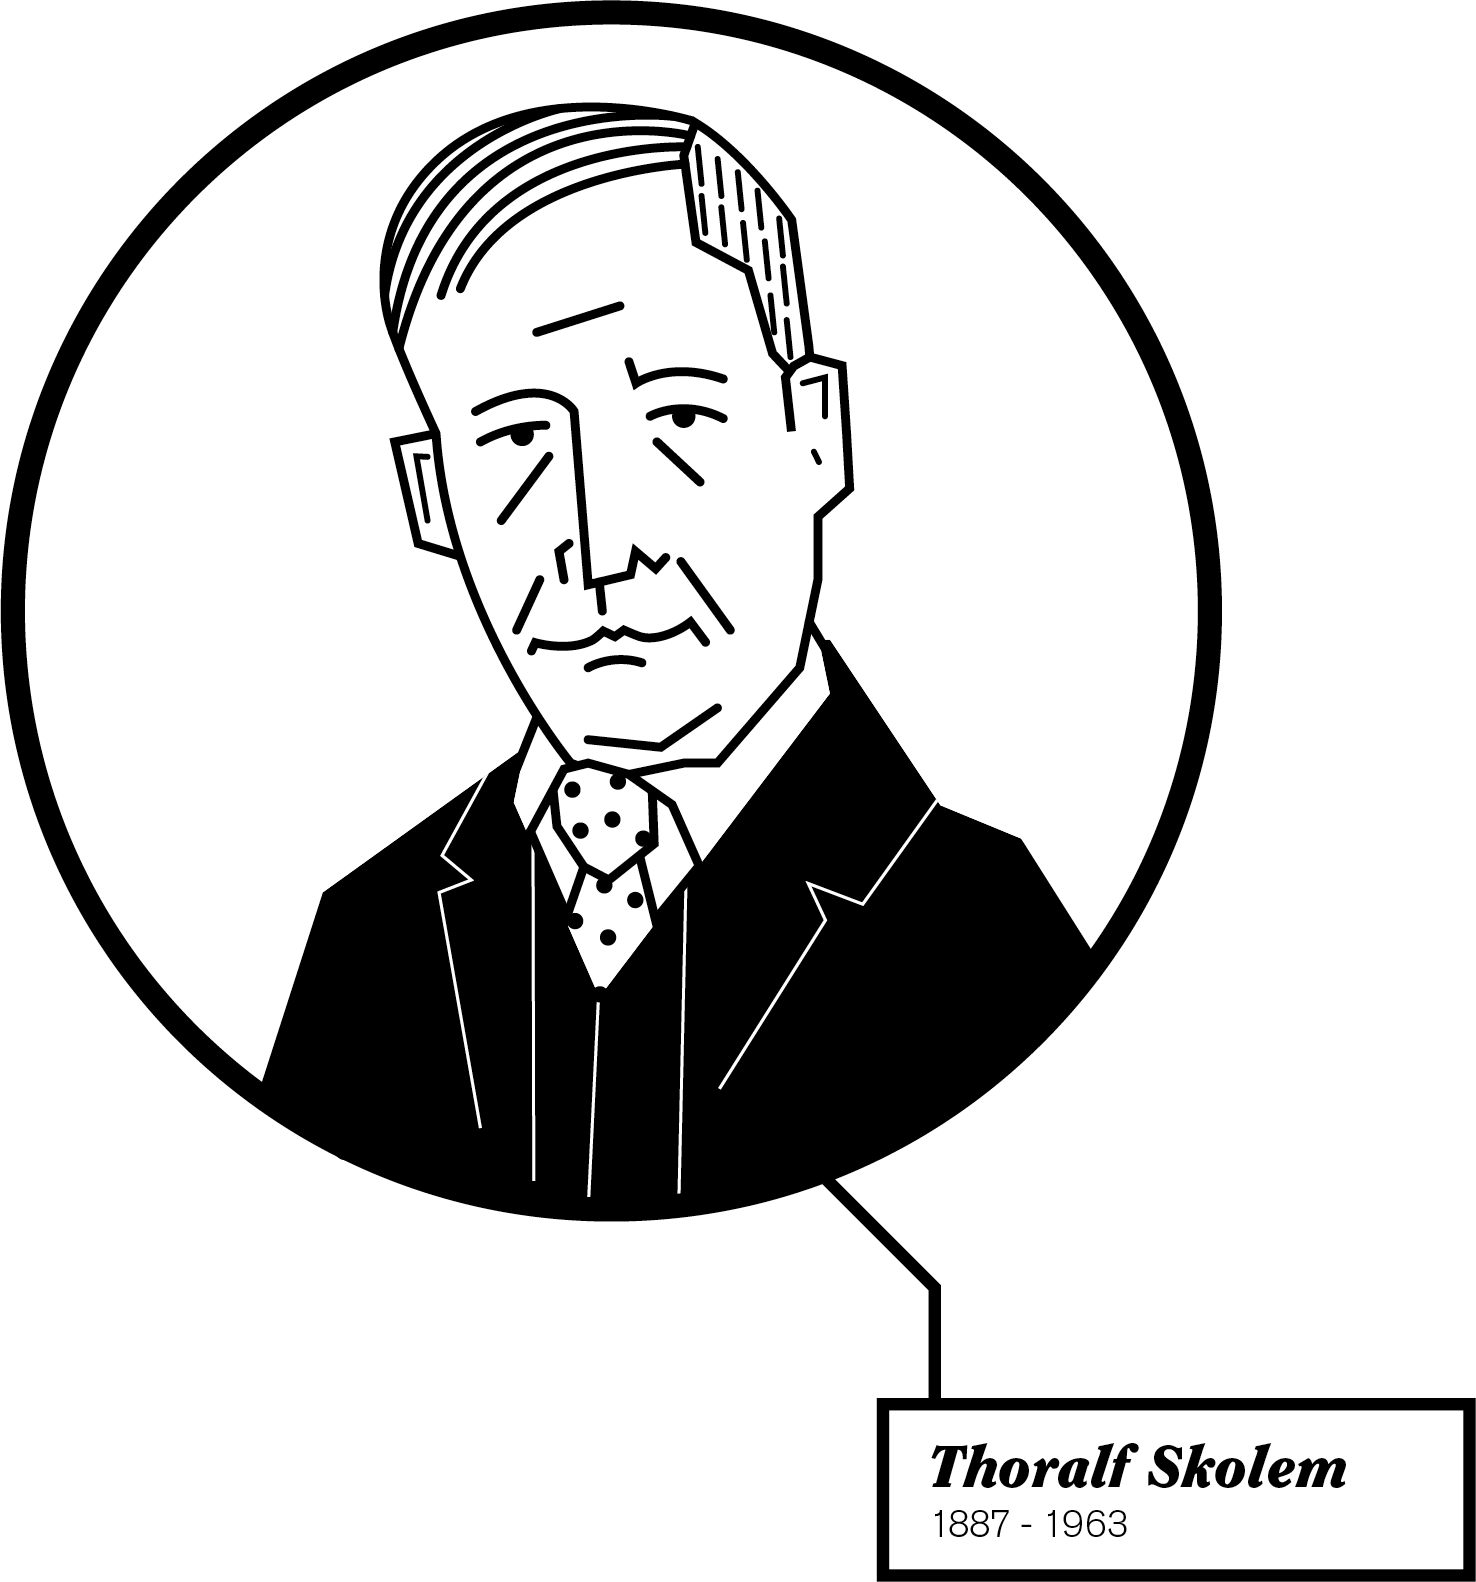
\includegraphics[width=\textwidth]{illustrations/SkolemChapter}
\vfill
\chapter{ভূমিকা}

বইটি অধিযুক্তিবিদ্যার পরিচয়, বিশেষ করে কম্পিউটার বিজ্ঞান ও দর্শনের
শিক্ষার্থীদের জন্য লেখা। যুক্তিবিদ্যাকেই যে শাস্ত্রের আলোচ্য বিষয় করা
হয়, তাকে সেই কারণেই বলা হয় ``অধিযুক্তিবিদ্যা''। যুক্তিবিদ্যার নিজের
আলোচ্য বিষয় বৈধ অনুমানের নিয়ম। তার সাংকেতিক বা বিধিবদ্ধ রূপে সেই
নিয়মগুলি প্রকাশ করতে বচনমূলক যুক্তিবিদ্যা ও প্রথম-ক্রমের যুক্তিবিদ্যার
ভাষার মতো বিধিবদ্ধ ভাষা ব্যবহার করা হয়। অধিযুক্তিবিদ্যায় এই ভাষাগুলির
ধর্ম এবং এই ভাষাগুলিকে কাজে লাগিয়ে সঠিক অনুমান করার নিয়মগুলির ধর্ম
বিচার করা হয়। বিধিবদ্ধ ভাষার রাশিগুলির অর্থ কীভাবে সুনির্দিষ্ট করা
যায়, বৈধ অনুমানের নিয়মগুলি কীভাবে সমর্থন করা যায় এবং বিভিন্ন
!!{derivation} পদ্ধতির কী কী ধর্ম আছে, যার মধ্যে গণনাসংক্রান্ত ধর্মও
পড়ে, এই সবই তার আলোচ্য। প্রশ্নগুলি নিজের গুণেই গুরুত্বপূর্ণ ও
কৌতূহলোদ্দীপক, কারণ আলোচ্য ভাষা ও !!{derivation} পদ্ধতিগুলি বহু
ক্ষেত্রে, বিশেষত গণিত, দর্শন, কম্পিউটার বিজ্ঞান ও ভাষাবিজ্ঞানে,
প্রয়োগ করা হয়। সেই সঙ্গে এগুলি দেখায়, সাধারণভাবে বিধিবদ্ধ পদ্ধতির
অধ্যয়ন কীভাবে করা যায়। এখানে যে যৌক্তিক ভাষাগুলি নিয়ে আলোচনা করব,
সেগুলি ছাড়াও আরও অনেক ভাষা নিয়ে আগ্রহ আছে। যেমন, বচনমূলক ও
প্রথম-ক্রমের যুক্তিবিদ্যার ভাষার চেয়ে অনেক জটিল ভাষা নিয়ে
ভাষাবিদ ও দার্শনিকদের আগ্রহ আছে। কম্পিউটার বিজ্ঞানীরা আবার একেবারে
অন্য \emph{ধরনের} ভাষা নিয়ে আগ্রহী, যেমন প্রোগ্রামিং ভাষা। বিধিবদ্ধ
ভাষার অর্থতত্ত্ব কীভাবে নির্দিষ্ট করা যায়, সেই ভাষা সম্পর্কে ফল কীভাবে
প্রমাণ করা যায়, তার ধর্ম কীভাবে অনুসন্ধান করা যায়, এই যে
পদ্ধতিগুলি নিয়ে আমরা আলোচনা করব, সেগুলি ওই ক্ষেত্রগুলিতেও প্রযোজ্য।

অন্য যে-কোনো শাস্ত্রের মতো অধিযুক্তিবিদ্যাতেও আছে কিছু
ফল বা তথ্য এবং সেগুলি নির্ণয় করার নানা পদ্ধতি ও কৌশল। এই বইয়ে
উভয়েরই আলোচনা আছে। অনেক শিক্ষার্থীর পাঠক্রমের বাইরে আমাদের
আলোচিত সব ফল জানার প্রয়োজন হবে না, কিন্তু যে পদ্ধতিতে আমরা
সেগুলি প্রতিষ্ঠা করি, সেই পদ্ধতিগুলি তাঁদের প্রয়োজন হবে এবং তাঁরা
সেগুলি কাজে লাগাবেন। যেমন, লোয়েনহাইম--স্কোলেম উপপাদ্য কম্পিউটার
বিজ্ঞানে সচরাচর দেখা যায় না, কিন্তু তার প্রমাণের পদ্ধতিগুলি দেখা
যায়। আবার আমাদের আলোচিত অনেক ফল বিজ্ঞানের দর্শন ও অধিবিদ্যার
কয়েকটি বিতর্কে প্রাসঙ্গিক। দর্শনের শিক্ষার্থীদের পাঠক্রমের বাইরে
হয়তো এই ফলগুলি প্রমাণ করার প্রয়োজন হবে না, কিন্তু ফলগুলি কী, তা
তাঁদের বুঝতে হবে। ফলগুলি প্রতিষ্ঠা করার জন্য প্রয়োজনীয় সংজ্ঞা ও
প্রমাণগুলি ভেবে দেখলেই কেবল সেগুলি সত্যি \emph{বোঝা} যায়। কম্পিউটার
বিজ্ঞান ও দর্শনের শিক্ষার্থীদের এই বইয়ের ফল ও পদ্ধতি অধ্যয়নের
পরামর্শ দেওয়া হয়, এমনকি কোনো কোনো ক্ষেত্রে তা আবশ্যিক।
এগুলি তার কয়েকটি কারণ।

বইয়ের বিষয়বস্তু তিনটি ভাগে বিভক্ত। \Olref[sfr][][]{part}-এ
সেটতত্ত্ব আলোচনা করা হয়েছে। ``গণিতের ভিত্তি'' নামে পরিচিত বিষয়টির
সঙ্গে যুক্তিবিদ্যা ও অধিযুক্তিবিদ্যার ঐতিহাসিক যোগ খুব ঘনিষ্ঠ।
পূর্ণসংখ্যা, মূলদ ও বাস্তব সংখ্যা, অপেক্ষক, স্থান ইত্যাদি গাণিতিক
বস্তু শেষ বিচারে কীভাবে বুঝতে হবে, গণিতের ভিত্তিতে সেই প্রশ্নটি
আলোচনা করা হয়। সেটতত্ত্ব তার একটি উত্তর দেয় (অন্য উত্তরও আছে),
তাই সেটতত্ত্ব ও যুক্তিবিদ্যা দীর্ঘকাল ধরে পাশাপাশি অধ্যয়ন করা হয়েছে।
গণিত, কম্পিউটার বিজ্ঞান ও দর্শনের অপেক্ষাকৃত কারিগরি কয়েকটি শাখা
সহ যে-কোনো বিধিবদ্ধ অনুসন্ধানে সেট, সম্পর্ক ও অপেক্ষকের ব্যবহার
সর্বত্র দেখা যায়। যুক্তিবিদ্যার অর্থতত্ত্ব ও প্রমাণতত্ত্ব এবং
গণনসাধ্যতার ভিত্তি সম্পর্কে ফল সূত্রবদ্ধ ও প্রমাণ করতে হলে
উপযুক্ত পরিভাষা থাকা অপরিহার্য। যেমন, আমরা রাশির সেট, অনুসিদ্ধান্ত
ও প্রমাণযোগ্যতার সম্পর্ক, বিধেয় সংকেতের ব্যাখ্যা (যেগুলি সম্পর্ক
বলে দেখা যাবে), গণনসাধ্য অপেক্ষক এবং এগুলির মধ্যে নানা সম্পর্ক ও
এগুলি ব্যবহার করে নানা নির্মাণের কথা বলব। এদের জন্য সংক্ষিপ্ত
সংকেত থাকলে সুবিধা হবে, আর সেট, সম্পর্ক ও অপেক্ষকের সাধারণ
ধর্মগুলিও ভেবে দেখা দরকার। গাণিতিকভাবে চিন্তা করা ও গাণিতিক প্রমাণ
সূত্রবদ্ধ করায় তোমার অভ্যাস না থাকলে, সেটতত্ত্বের প্রথম ভাগটিকে
অনুশীলনের ক্ষেত্র বলে ধরে নাও। সেখানে মৌলিক সংজ্ঞাগুলি সবই দেওয়া
হবে এবং সেগুলি কাজে লাগিয়ে ক্রমশ আরও জটিল প্রমাণ দেওয়া হবে।
বিশেষত প্রথম ভাগে ফল বোঝার চেয়েও হয়তো বেশি জরুরি এই প্রমাণগুলি
বোঝা এবং নিজে প্রমাণ খুঁজে বার করে সূত্রবদ্ধ করতে পারা। গাণিতিক
চিন্তায় তুমি নতুন হলে উদাহরণ ও সমস্যাগুলি ভালো করে ভেবে দেখো।

তবে প্রথম ভাগে আমরা একটি গুরুত্বপূর্ণ ফল প্রতিষ্ঠা করব। কান্টরের
উপপাদ্য নামে পরিচিত এই ফলটি নির্ভর করে কান্টরের অসীমতার বিশ্লেষণের
উপর, যা বিজ্ঞানের যে-কোনো শাখায় ধারণা-বিশ্লেষণের সবচেয়ে চমকপ্রদ
দৃষ্টান্তগুলির একটি। অসীমতা শত শত বছর ধরে গণিতবিদ ও দার্শনিক
উভয়কেই ভাবিয়েছে। কান্টরের আগে কেউ জানতেন না কীভাবে বিষয়টি
ঠিকমতো ভাবতে হয়। এমনকি অনেকে মনে করতেন, অসীমতা নিয়ে চিন্তা
করাটাই ভুল, আর অসীম সমষ্টির ধারণাটিই অসংগত। কান্টর অসীমতাকে
এমন একটি বিষয় করে তুললেন যা নিয়ে সঙ্গতভাবে কাজ করা যায়। তিনি
অসীম সমষ্টির একটি পূর্ণাঙ্গ তত্ত্ব গড়ে তুললেন, সেই সঙ্গে এমন অসীম
সংখ্যার তত্ত্বও, যা দিয়ে অসীম সমষ্টির আকার মাপা যায়। তিনি দেখালেন,
অসীমতার বিভিন্ন স্তর আছে। ``ট্রান্সফাইনাইট'' সংখ্যার এই তত্ত্ব
সুন্দর ও জটিল। আমরা তার খুব গভীরে যাব না, তবে অসীমতার যে বিভিন্ন
স্তর আছে, তা দেখাতে পারব। বিশেষ করে অসীমতার ``গণনীয়'' ও
``অগণনীয়'' স্তর দেখব। এই ফলের গুরুত্বপূর্ণ প্রয়োগ আছে, আর
নিজের বিদ্যাকে মর্যাদা দেন এমন যে-কোনো গণিতবিদ, কম্পিউটার বিজ্ঞানী
ও দার্শনিকেরই এ ধরনের ফল জানা উচিত।

\olref[fol][][]{part}-এ আমরা প্রথম-ক্রমের যুক্তিবিদ্যার আলোচনায় আসব।
প্রথম-ক্রমের যুক্তিবিদ্যার ভাষা ও তার অর্থতত্ত্ব সংজ্ঞায়িত করব,
অর্থাৎ প্রথম-ক্রমের গঠন কী এবং কোনো গঠনে প্রথম-ক্রমের যুক্তিবিদ্যার
একটি বাক্য কখন সত্য হয়, তা বলব। এতে আমরা দুটি গুরুত্বপূর্ণ কাজ
করতে পারব। (১)~একটি বাক্য কখন আর-একটি বাক্যের যৌক্তিক অনুসিদ্ধান্ত,
তা গাণিতিক নির্ভুলতায় সংজ্ঞায়িত করতে পারব। (২)~প্রথম-ক্রমের
গঠন যে সম্পর্কগুলি নিয়ে তৈরি, সেই গঠনে সত্য বাক্যগুলি কীভাবে
সম্পর্কগুলিকে বর্ণনা করে, অর্থাৎ চরিত্রায়িত করে, তাও বিচার করতে
পারব। বিশেষ করে এখান থেকেই আমরা স্বতঃসিদ্ধমূলক পদ্ধতির আলোচনায়
পৌঁছব। এই পদ্ধতিতে প্রথম-ক্রমের ভাষার বাক্য ব্যবহার করে কয়েক ধরনের
গঠনকে চরিত্রায়িত করা হয়। তার পরে প্রমাণতত্ত্ব নিয়ে আলোচনা করব।
১৯৩০-এর দশকে গেরহার্ড গেৎসেন যে সিকোয়েন্ট কলন ও স্বাভাবিক
নিষ্পাদনের সংজ্ঞা দিয়েছিলেন, আমরা তাদের আদি রূপগুলি বিবেচনা করব।
(তোমাদের শিক্ষক হয়তো পদ্ধতি দুটির একটি মাত্র পড়াবেন। সে ক্ষেত্রে
``!!{derivation}s'' এবং ``!!{derivability}'' যেখানে বলা হয়েছে,
সেখানে তাঁর বেছে নেওয়া পদ্ধতিটিই বোঝাবে।) অনুসিদ্ধান্তের অর্থগত
ধারণা ও !!{derivability}-র সংকেতবিন্যাসগত ধারণা কয়েকটি বাক্য
থেকে আর-একটি বাক্য অনুসৃত হওয়ার কথাটিকে নির্ভুল করার দুটি
সম্পূর্ণ ভিন্ন উপায় দেয়। বিশুদ্ধতা ও পূর্ণতা উপপাদ্য এই দুটি
চরিত্রায়নকে যুক্ত করে। বিশেষ করে আমরা গ্যোডেলের পূর্ণতা উপপাদ্য
প্রমাণ করব। উপপাদ্যটি বলে, একটি বাক্য কয়েকটি বাক্যের অর্থগত
অনুসিদ্ধান্ত হলে সেটি সেগুলি থেকে !!{derivable}-ও হয়। কথাটি
সমতুল্যভাবে এই রকম। বাক্যের একটি সমষ্টি সঙ্গত হলে, অর্থাৎ তা থেকে
কোনো বিরোধ প্রমাণ করা না গেলে, এমন একটি গঠন আছে যাতে সব
বাক্যই সত্য।

পূর্ণতা উপপাদ্যের দ্বিতীয় রূপটিই হয়তো বেশি বিস্ময়কর। গ্যোডেল
যে সময়ে এই ফলটি প্রমাণ করেন (১৯২৯ সালে), তার কাছাকাছি সময়ে
জার্মান গণিতবিদ ডাভিড হিলবার্টের একটি বিখ্যাত মত ছিল যে গাণিতিক
অস্তিত্বের জন্য সঙ্গতিই যথেষ্ট, অর্থাৎ বিরোধ না থাকলেই চলে।
অন্যভাবে বললে, কোনো গণিতবিদ একটি গঠন বা এক শ্রেণির গঠন সঙ্গতভাবে
বর্ণনা করতে পারলেই এমন গঠনের অস্তিত্বে বিশ্বাস করার অধিকার তাঁর
থাকা উচিত। সে সময় অনেকে এই ধারণাকে উদ্ভট মনে করতেন। নিজেই
নিজের কথার বিরোধ না ঘটিয়ে তুমি একটি গঠন বর্ণনা করতে পারছ বলেই
যে এমন গঠন সত্যিই আছে, তা নিশ্চয়ই অনুসৃত হয় না। অথচ গ্যোডেলের
পূর্ণতা উপপাদ্য ঠিক এই কথাই বলে। পূর্ণতা উপপাদ্যের এই আপাত
বিরোধময় দিকটি দর্শনের দিক থেকেও যথেষ্ট কৌতূহল জাগায়। এর দুটি
গুরুত্বপূর্ণ প্রয়োগও আছে, যা দিয়ে প্রদত্ত বাক্যগুলিকে সত্য করে
এমন গঠনের অস্তিত্ব সম্পর্কে আরও ফল প্রমাণ করা যায়। এগুলি হলো
সংহতি উপপাদ্য এবং লোয়েনহাইম--স্কোলেম উপপাদ্য।

\olref[tur][][]{part}-এ যুক্তিবিদ্যার সঙ্গে গণনসাধ্যতার যোগ স্থাপন
করব। এখানেও একটি ঐতিহাসিক যোগ আছে। ডাভিড হিলবার্ট যুক্তিবিদ্যার
মৌলিক সমস্যা হিসেবে এই প্রশ্নটি তুলেছিলেন। যুক্তিবিদ্যার একটি
বাক্য দেওয়া থাকলে সেটি প্রমাণ করা যায় কি না, তা নির্ণয়ের কোনো
যান্ত্রিক পদ্ধতি কি পাওয়া যায়? বচনমূলক যুক্তিবিদ্যার ক্ষেত্রে
অবশ্য এমন পদ্ধতি আছে। শুধু সব সত্যসারণি পরীক্ষা করতে হয়, আর
তাদের সংখ্যা সসীম বলে পদ্ধতিটি একসময় সঠিক উত্তর দেয়। প্রথম-ক্রমের
যুক্তিবিদ্যায় এমন সরল পদ্ধতি সম্ভব নয়, কারণ সম্ভাব্য গঠনের সংখ্যা
অসীম (গঠনগুলিও নিজেরা অসীম হতে পারে)। যুক্তিবিদরা বছরের পর বছর
ধরে আরও কৌশলী পদ্ধতি খুঁজেছিলেন। শেষ পর্যন্ত অ্যালোনজো চার্চ ও
অ্যালান টুরিং প্রতিষ্ঠা করেন যে এমন কোনো পদ্ধতিই নেই। তা দেখাতে
প্রথমেই সাধারণভাবে যান্ত্রিক পদ্ধতি বলতে কী বোঝায়, তার সুনির্দিষ্ট
সংজ্ঞা দেওয়া দরকার ছিল। কোনো নির্ণয়পদ্ধতি প্রস্তাব করা হলে সম্ভবত
সেটিকে কার্যকর পদ্ধতি বলে চেনা যেত। কার্যকর পদ্ধতির অস্তিত্ব নেই
প্রমাণ করতে গেলে প্রথমে ``কার্যকর পদ্ধতি'' সংজ্ঞায়িত করে, সেই
সংজ্ঞার ভিত্তিতে অসম্ভাব্যতা প্রমাণ করতে হবে। টুরিং ঠিক তা-ই
করেছিলেন। একটি যান্ত্রিক পদ্ধতি নীতিগতভাবে কী করতে পারে, তার
গাণিতিক মডেল হিসেবে তিনি একটি টুরিং
যন্ত্রের\footnote{টুরিং নিজে অবশ্য একে এই নামে ডাকেননি।} ধারণা প্রস্তাব
করেন। গাণিতিক উপকরণ ব্যবহার করে একটি অনানুষ্ঠানিক ধারণার
\emph{ধারণাগত বিশ্লেষণ} করার এটি আর-একটি উদাহরণ। গণিতের পক্ষে
কান্টরের অসীমতার বিশ্লেষণ যতটা গুরুত্বপূর্ণ, কম্পিউটার বিজ্ঞানের
পক্ষে এই বিশ্লেষণ হয়তো ততটাই গুরুত্বপূর্ণ। আমাদের শেষ বড় কাজ
হবে অসম্ভাব্যতার দুটি উপপাদ্য প্রমাণ করা। আমরা দেখাব, টুরিং
যন্ত্র দিয়ে তথাকথিত ``থামার সমস্যা'' সমাধান করা যায় না এবং শেষে
দেখাব, হিলবার্টের ``সিদ্ধান্ত সমস্যা''-রও (যুক্তিবিদ্যার জন্য)
সমাধান করা যায় না।

বইটি গাণিতিক এই অর্থে যে আমরা গাণিতিক সংজ্ঞা আলোচনা করি এবং
আমাদের ফলগুলি গাণিতিকভাবে প্রমাণ করি। তবে এর জন্য গণিতের
বিস্তৃত পূর্বজ্ঞান দরকার হয় না। বইয়ের কোনো অংশ বুঝতেই
বীজগণিত, ত্রিকোণমিতি বা ক্যালকুলাস জানতে হবে না। গণিতে কীভাবে কাজ
করা হয়, তার সঙ্গেও যাতে আগে থেকে পরিচয় না লাগে, সে দিকে আমরা
বিশেষ নজর দিয়েছি। আসলে, আমাদের ফলগুলি বুঝতে ও প্রমাণ করতে যে
ধরনের যুক্তি ও প্রমাণের দক্ষতা দরকার, তা \emph{গড়ে তোলা} এই
বইয়ের একটি উদ্দেশ্য। বইয়ের বিন্যাস গাণিতিক রীতি অনুসরণ করে।
এর কারণ স্পষ্টতা ও নির্ভুলতা গণিতে বিশেষভাবে গুরুত্বপূর্ণ বলেই
এই রীতিগুলি গড়ে উঠেছে। যেমন, কোনো কথা একটি যুক্তির সিদ্ধান্ত
হিসেবে বলা হচ্ছে, অন্য কিছুর পক্ষে কারণ হিসেবে দেওয়া হচ্ছে, না
নতুন পরিভাষা পরিচয় করিয়ে দিতে বলা হচ্ছে, তা বোঝা জরুরি। তাই
গাণিতিক রীতি মেনে নতুন পরিভাষা বা সংকেত পরিচয় করিয়ে দেওয়ার
অংশগুলিকে ``সংজ্ঞা'' বলব, আর কোনো ফল বা প্রাপ্ত তথ্য লিপিবদ্ধ করার
সময় ``উপপাদ্য'', ``প্রতিজ্ঞা'', ``সহায়ক উপপাদ্য'' বা
``অনুসিদ্ধান্ত'' আখ্যা ব্যবহার করব। এই রীতিগুলি ছাড়াও আমরা
যৌক্তিক প্রমাণের সেই পদ্ধতিগুলি ব্যবহার করব যার সঙ্গে প্রথম
যুক্তিবিদ্যার পাঠক্রমেই হয়তো তোমাদের পরিচয় হয়েছে। ফল প্রমাণে
\emph{গাণিতিক আরোহ} পদ্ধতিও ব্যাপকভাবে ব্যবহার করব। পরিশিষ্টের
দুটি অধ্যায় এই প্রমাণপদ্ধতিগুলি নিয়ে।

\paragraph{শিক্ষকদের জন্য কয়েকটি কথা} এই বইয়ের বিষয়বস্তু
বিধিবদ্ধ যুক্তিবিদ্যার এক সেমেস্টারের দ্বিতীয় পাঠক্রমের
উপযোগী। ক্যালগেরি বিশ্ববিদ্যালয়ে আমি যুক্তিবিদ্যা~২ পাঠক্রমে
১২ সপ্তাহে এটি পড়াই, যদিও বইয়ে যতটা বিস্তারিত আলোচনা আছে, সব
বিষয় ততটা খুঁটিয়ে পড়াই না। যেমন, সাধারণত আমি শুধু স্বাভাবিক
নিষ্পাদন নিয়ে আলোচনা করি এবং অভিন্নতাসহ পূর্ণতার বিস্তারিত
প্রমাণগুলি বাদ দিই। শিক্ষার্থীরা আগেই যুক্তিবিদ্যা~১ পড়েছে।
সেই পাঠক্রমে সাধারণত
\emph{\href{https://forallx.openlogicproject.org}{forall x: Calgary}}
বইটি পড়ানো হয়। সেখানে স্বাভাবিক নিষ্পাদনের একই বিধিগুলি ব্যবহার
করা হয়, তবে ফিচের বিন্যাসে।

বইটির ইংরেজি সংস্করণের সর্বশেষ পিডিএফ
\href{https://slc.openlogicproject.org}{slc.openlogicproject.org}-এ
পাওয়া যায়, তবে বইটিতে ঘন ঘন পরিবর্তন হয়। সিসি বিওয়াই লাইসেন্সে
আপনি নিজেই বইটি ডাউনলোড ও বিতরণ করতে পারেন। যে সেমেস্টারে বইটি
ব্যবহার করবেন, তার পুরোটা জুড়ে সব শিক্ষার্থীর কাছে বইটির একই
সংস্করণ রাখতে এভাবেই বিতরণ করুন। শিক্ষার্থীদের শুধু লিঙ্ক না দিয়ে
যে পিডিএফটি ব্যবহার করতে চান, সেটি আপনার শিক্ষণ ব্যবস্থাপনা
প্রণালীতে আপলোড করুন। আপনার বইয়ের দোকান থেকেও পিডিএফগুলি
ছাপিয়ে নিতে পারেন। তবে কোনো কোনো দোকান অ্যামাজনে পাওয়া
পেপারব্যাক বই কিনে মজুত রাখতে পারবে।

প্রথম-ক্রমের যুক্তিবিদ্যার সংকেতবিন্যাস, অর্থতত্ত্ব ও প্রমাণপদ্ধতি
শেখাতে গ্রাহাম লিচ-ক্রাউসের বিনামূল্যের অনলাইন যুক্তিবিদ্যা-শিক্ষণ
সফটওয়্যার \emph{Carnap}
(\href{https://carnap.io}{carnap.io}) ব্যবহার করা যায়। স্বাভাবিক
নিষ্পাদন ও সিকোয়েন্ট কলনের !!{derivation}s, সরল তত্ত্বের জন্য গঠন
নির্দিষ্ট করা এবং সংকেতে প্রকাশ করার মতো অনুশীলনী এতে জমা দেওয়া
যায় ও স্বয়ংক্রিয়ভাবে মূল্যায়ন করা হয়। এ ছাড়া
\href{https://turing.openlogicproject.org}{turing.openlogicproject.org}-এ
একটি টুরিং যন্ত্র সিমুলেটর আছে। \olref[tur][][]{part}-এর আলোচ্য
বিষয়গুলি দেখাতে সেটি ব্যবহার করা যায়। ওই ভাগের উদাহরণগুলি
সিমুলেটরে আগে থেকেই দেওয়া আছে।

\cleartoverso
\thispagestyle{empty}
\ \vfill
\noindent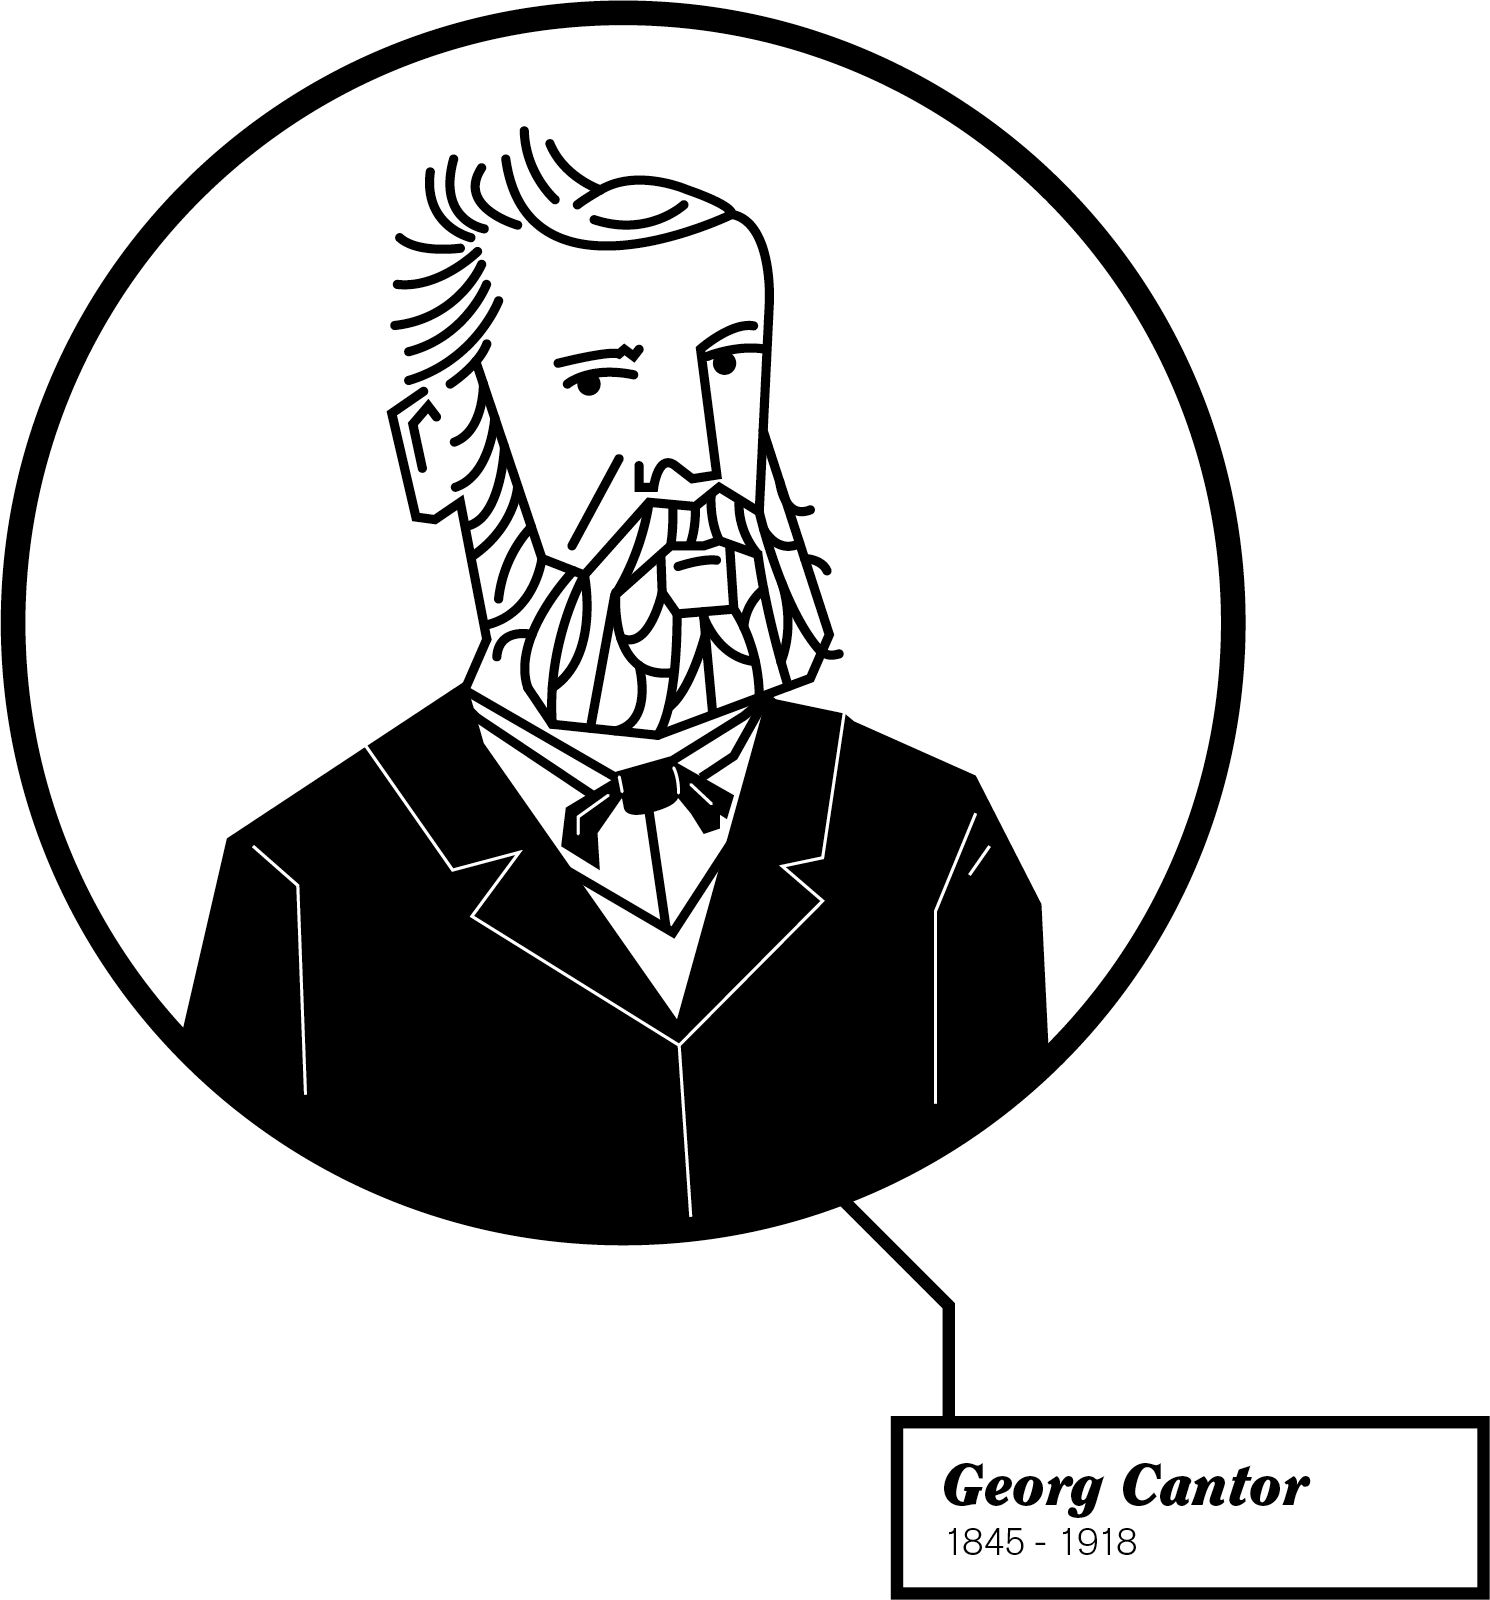
\includegraphics[width=\textwidth]{illustrations/CantorChapter}
\vfill
\mainmatter
\olimport*[sets-functions-relations]{sets-functions-relations}
\cleartoverso
\ifodd\value{page}\stepcounter{page}\fi
\thispagestyle{empty}
\ \vfill
\noindent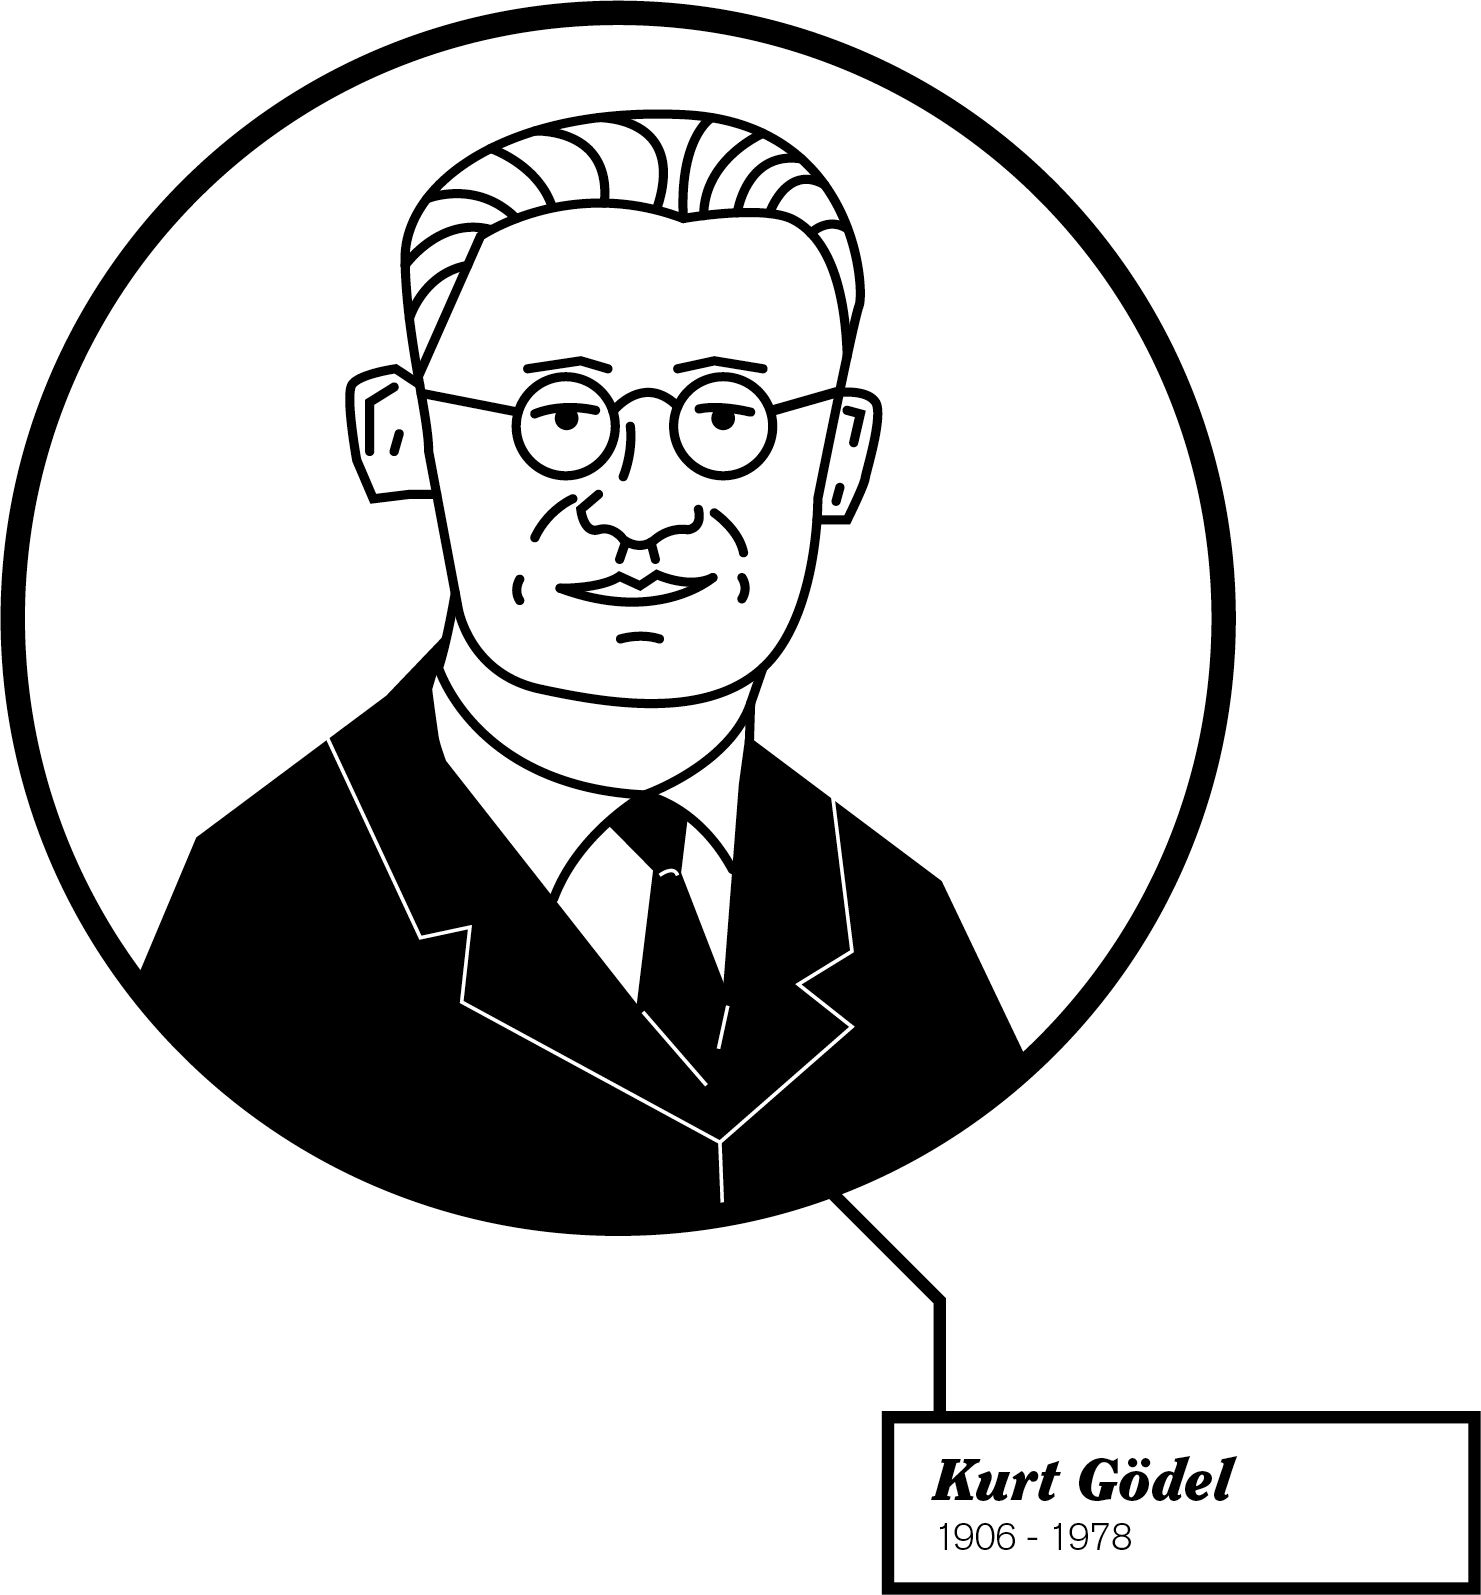
\includegraphics[width=\textwidth]{illustrations/GodelChapter}
\vfill
\olimport*[first-order-logic]{first-order-logic}
\cleartoverso
\ifodd\value{page}\stepcounter{page}\fi
\thispagestyle{empty}
\ \vfill
\noindent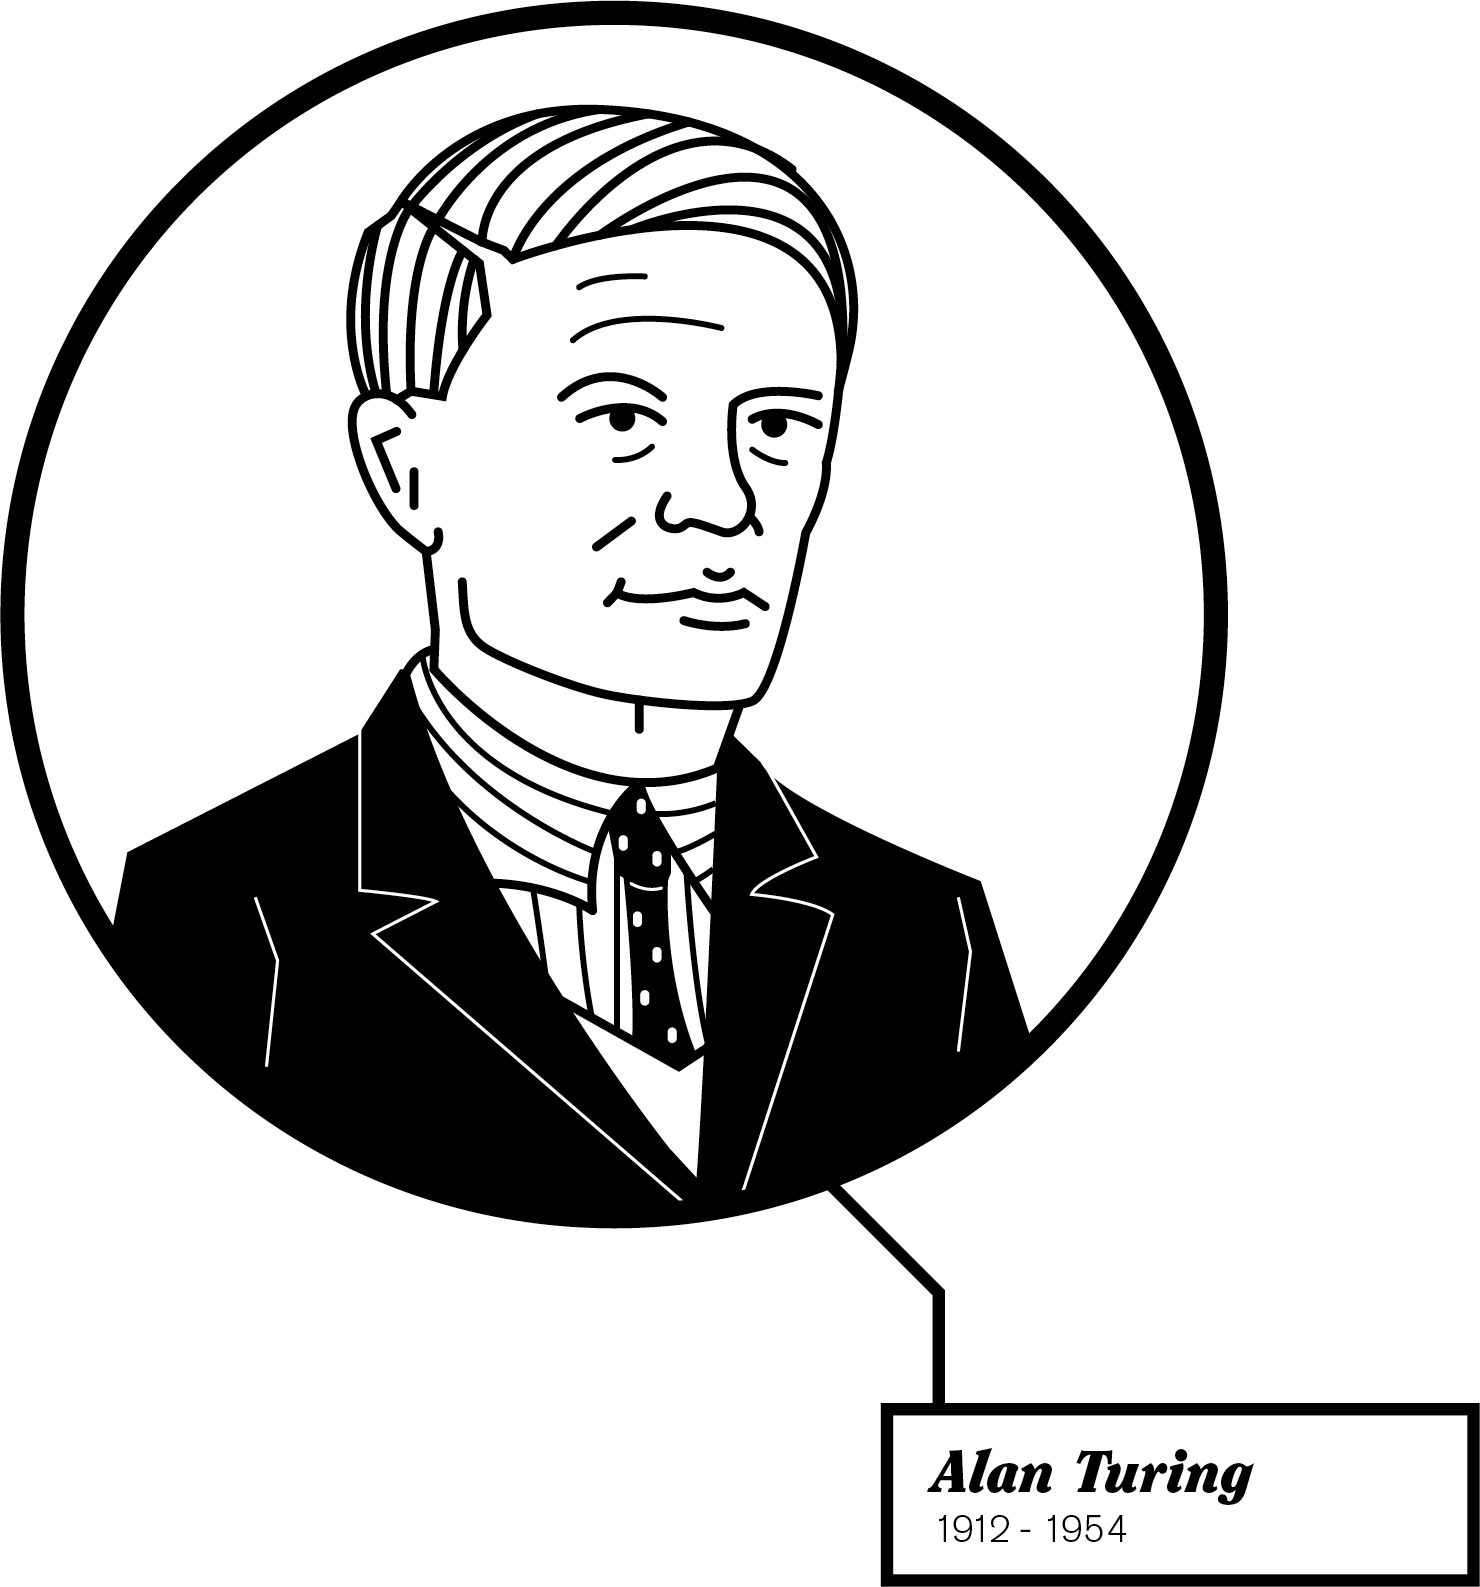
\includegraphics[width=\textwidth]{illustrations/TuringChapter}
\vfill
\olimport*[turing-machines]{turing-machines}
\cleartoverso
\ifodd\value{page}\stepcounter{page}\fi
\thispagestyle{empty}
\ \vfill
\noindent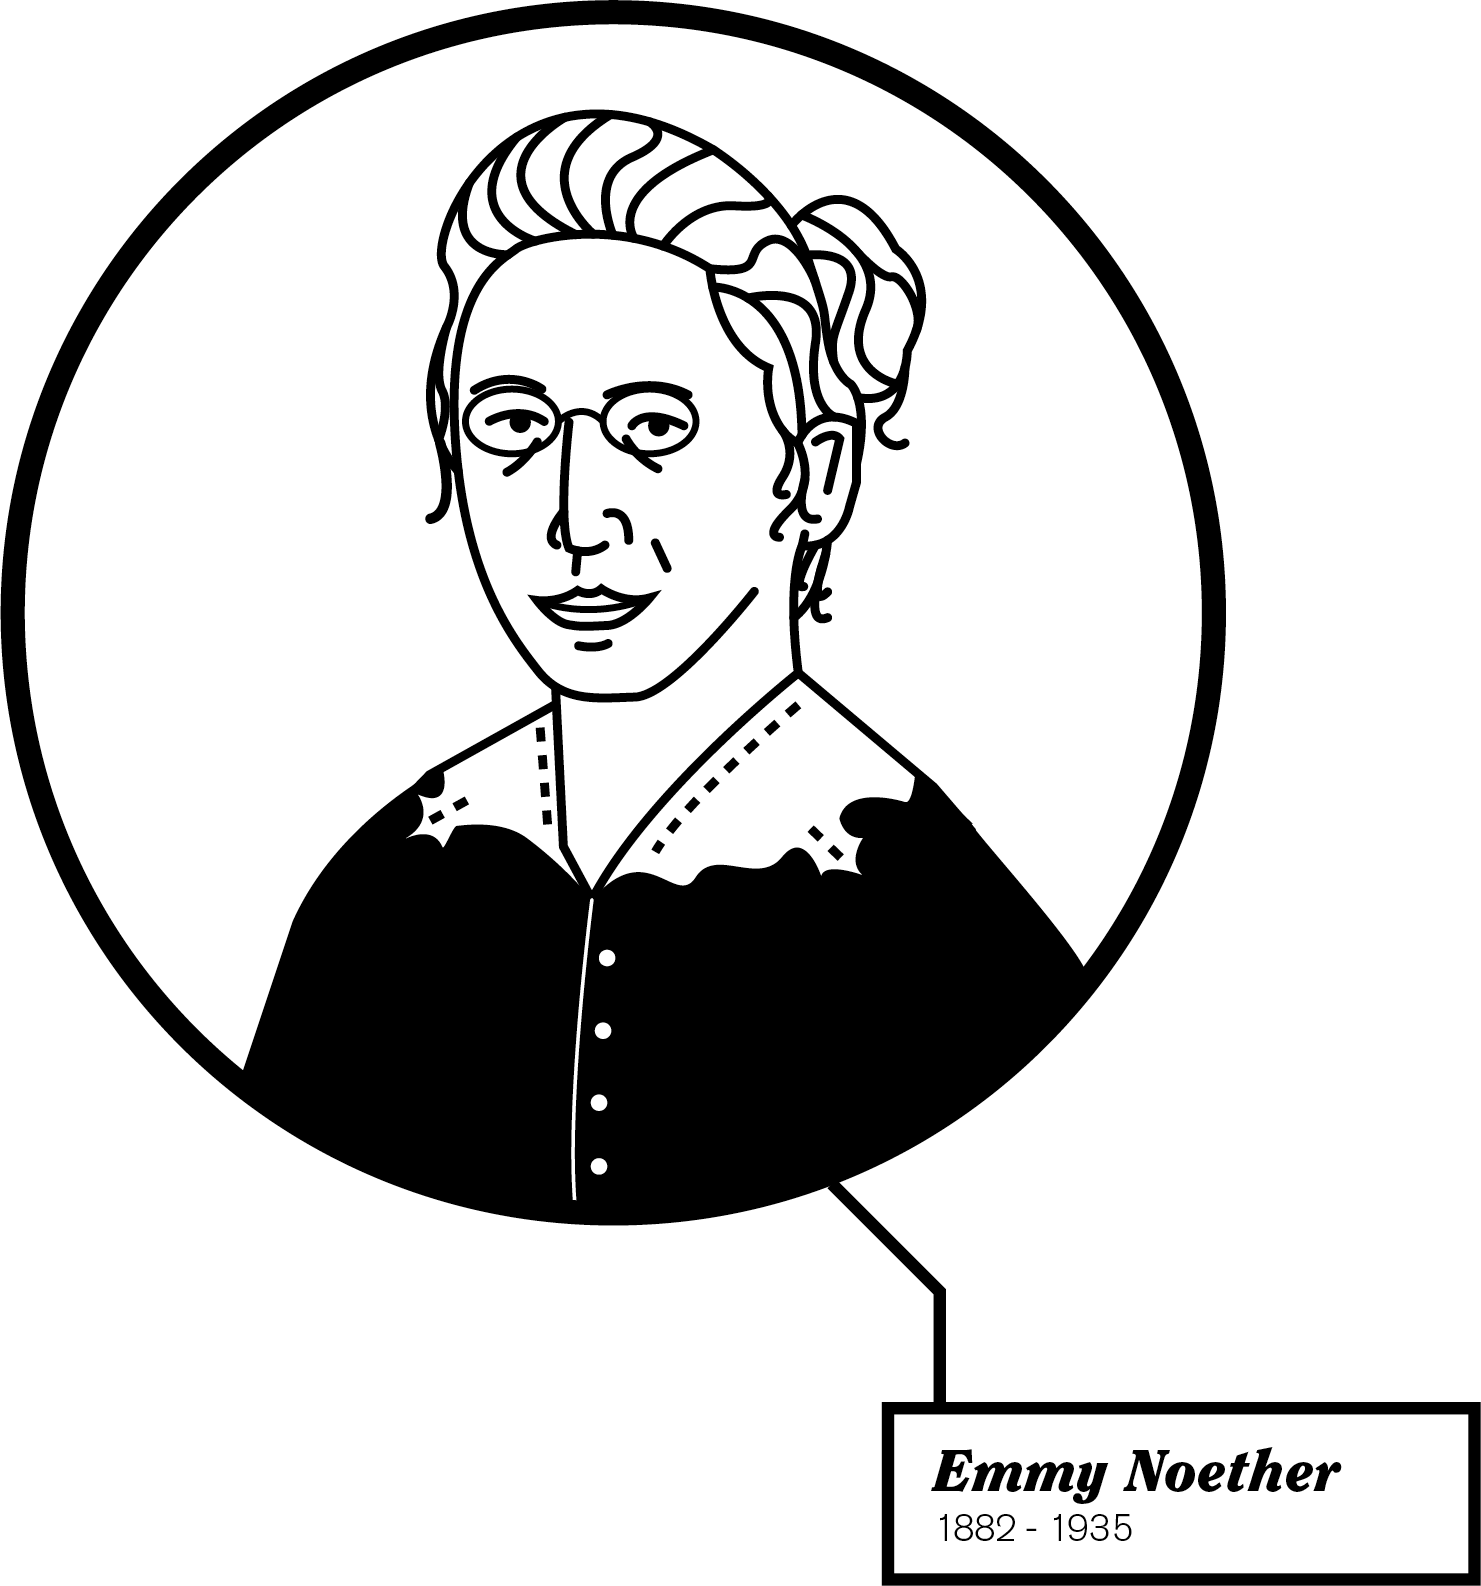
\includegraphics[width=\textwidth]{illustrations/NoetherChapter}
\vfill
\appendix
\olimport*[methods/proofs]{proofs}
\olimport*[methods/induction]{induction}
\stopproblems
\def\ifproblems#1{}
\def\figurename{চিত্র}
\setlength{\olphotowidth}{.45\textwidth}
\chapter{জীবনী}
\olimport*[history/biographies]{georg-cantor}
\olimport*[history/biographies]{alonzo-church}
\olimport*[history/biographies]{gerhard-gentzen}
\olimport*[history/biographies]{kurt-goedel}
\olimport*[history/biographies]{emmy-noether}
\olimport*[history/biographies]{bertrand-russell}
\olimport*[history/biographies]{alfred-tarski}
\olimport*[history/biographies]{alan-turing}
\olimport*[history/biographies]{ernst-zermelo}
\olimport*[reference/greek-alphabet]{greek-alphabet}
\glsaddall
\printglossary[title={পরিভাষাকোষ},toctitle={পরিভাষাকোষ}]
\clearpage
\photocredits
\bibliographystyle{natbib-oup}
\bibliography{\olpath/bib/open-logic}
\olimport*{\olpath/locale/\ollangid/content/open-logic-about}

\end{document}
